\documentclass[../../main.tex]{subfiles}

\begin{document}
\section{Dinamica}
\subsection{Concetto di forza}
La forza è la grandezza che esprime e misura l'interazione tra sistemi fisici.
\subsection{Primo principio della dinamica: principio d'inerzia}
Un corpo non soggetto a forze si muove di moto rettilineo uniforme oppure sta fermo se inizialmente era fermo. $\bar v =$ costante.
\subsection{Secondo principio della dinamica: principio fondamentale della dinamica}
La variazione di quantità di moto di un corpo è proporzionale alla forza impressa e avviene nella direzione della forza stessa. \[\bar F = m \bar a.\]
L'accelerazione è sempre nella direzione della forza, e il rapporto delle accelerazioni è inverso al rapporto delle masse:
\[
    \begin{array}{lr}
        F = m_1 a_1 \\
        F = m_2 a_2
    \end{array} = m_1 a_1 = m_2 a_2 \implies \frac{a_1}{a_2} = \frac{m_2}{m_1}
\]

\subsubsection{Massa di un corpo}
La massa si misura con la bilancia. La forza della gravità è proporzionale alla massa del corpo:
\[
    \bar F = m \bar g
\]
\subsection{Seconda legge di Newton}
Esprime la legge fondamentale della dinamica del punto:
\[
    \bar F = m\bar{a} = m\dfrac{d\bar v}{dt} = m\dfrac{d^2\bar{r}}{dt^2} \ \ \ \star
\]
Possiamo scrivere $\star$ scomponendola in tre equazioni relative ai tre moti proiettati sugli assi cartesiani:
\[
    \begin{cases}
        F_x = m\bar{a}_x = m\dfrac{d^2x}{dt^2} \\
        \vspace{1px}                           \\
        F_y = m\bar{a}_y = m\dfrac{d^2y}{dt^2} \\
        \vspace{1px}                           \\
        F_z = m\bar{a}_z = m\dfrac{d^2z}{dt^2}
    \end{cases}
\]
\subsection{Terza legge della dinamica}
Immaginiamo di avere due corpi A e B: se A esercita una forza su B, allora B esercita una forza uguale e opposta su A, \textbf{principio di azione e reazione.}\\
\begin{minipage}{0.5\textwidth}
    \centering
    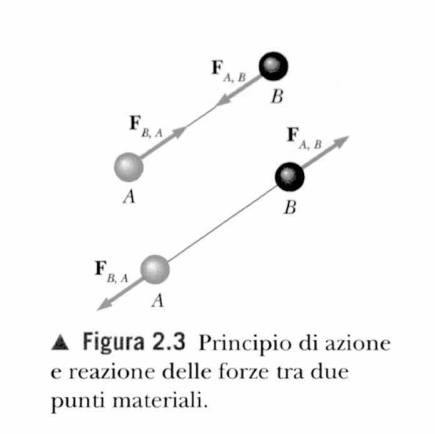
\includegraphics[width=0.5\textwidth]{reazioneazione.png}
\end{minipage}
\begin{minipage}{0.5\textwidth}
    \centering
    \[\bar F_{AB} = -\bar F_{BA}\]
\end{minipage}
\begin{center}
    \textit{Ad ogni azione corrisponde una reazione uguale e contraria.}\\
\end{center}
Se A e B sono la Terra e il sole allora:
\[
    F = G \dfrac{M_t M_s}{r^2} \ \ \ \textit{Gravitazione}
\]
Per le cariche:
\[
    F = k \dfrac{q_1 q_2}{r^2} \ \ \ \textit{Elettromagnetica}
\]
Questo non significa che i due corpi non si muovano, anzi si muovono in qundo il punto di applicazione è diverso: immagina la roulotte e la macchina.
\subsection{Quantità di moto, impulso}
Si definisce quantità di moto di un punto materiale il vettore:
\[
    \bar p = m\bar v
\]
Se la massa è costante la seconda legge di Newton diventa:
\[
    \bar F = \dfrac{d\bar p}{dt}
\]
Da cui si ottiene il teorema dell'impulso:
\[
    \bar F dt = d\bar p \implies \int_{0}^{t_0} \bar F dt = \int_{\bar p_i}^{\bar p_f} d\bar p = \bar p_f - \bar p_i = \Delta\bar p = \bar J
\]
Dove $\bar J$ è l'impulso della forza $\bar F$ e $\Delta p$ è la variazione della quantità di moto. . Il teorema dell'impulso dice che:\\
\textit{l'impulso do una forza applicata a un punto materiale provoca la variazione della quantità di moto}\\
Se la massa è costante:
\[
    \bar F_m \cdot \Delta t = \Delta \bar p \implies \bar F_m = \dfrac{\Delta\bar p}{\Delta t}
\]
\subsubsection{Unità di misura}
\[
    [\bar F] = [M]\cdot\dfrac{[L]}{[T^2]} \implies \dfrac{kg\cdot m}{s^2} = N
\]
\[
    [\bar p] = [M]\cdot\dfrac{[L]}{[T]} \implies \dfrac{kg\cdot m}{s} = N\cdot s
\]
\subsubsection{Esercizio 2.1}
\begin{figure}[H]
    \centering
    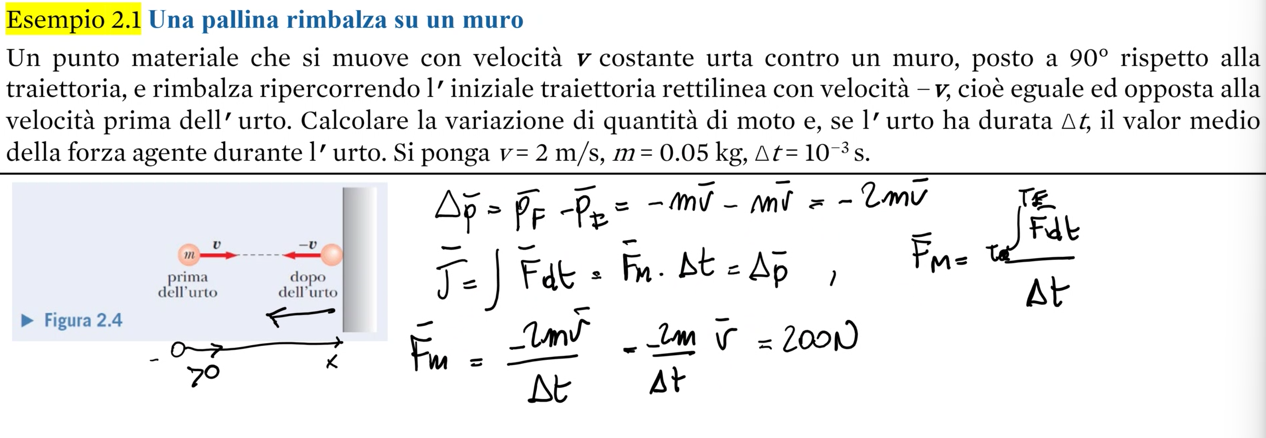
\includegraphics[width=0.7\textwidth]{2-1.png}
\end{figure}

\subsection{Risultante delle forze, equilibrio statico}
\begin{minipage}
    {0.5\textwidth}
    \centering
    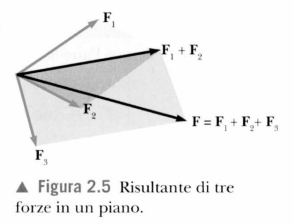
\includegraphics[width=0.5\textwidth]{3forze.png}
\end{minipage}
\begin{minipage}{0.5\textwidth}
    \centering
    Principio di sovrapposizione:\\
    \[
        \bar F = \bar F_1 + \bar F_2 + \bar F_3 + \ldots + \bar F_n = \sum_{i=1}^{n} \bar F_i
    \]
\end{minipage}
e l'accelerazione del punto è pari alla somma vettoriale delle accelerazioni che il punto avrebbe se agisse ciascuna forza separatamente:
\[
    \bar a = \dfrac{\bar F}{m}
\]
\textbf{indipendenza delle azioni simultanee}.\\
Se $\bar F = 0$ e $\bar v = 0$ allora il punto rimane in quiete: sono realizzate le condizioni di equilibrio statico. Devono quindi essere nulle tutte le componenti della risultate ovvero con riferimento a un sistema di assi cartesiani:
\[
    \bar F = \sum_{i} \bar F_i = 0 \implies \begin{cases}
        F_x = \sum_i F_{ix} = 0 \\
        F_y = \sum_i F_{iy} = 0 \\
        F_z = \sum_i F_{iz} = 0
    \end{cases}
\]
\begin{figure}[H]
    \centering
    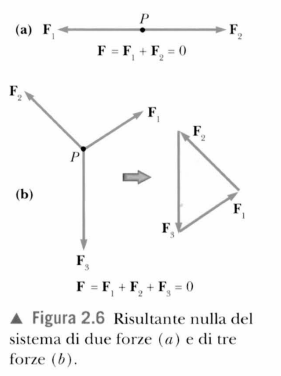
\includegraphics[width=0.3\textwidth]{eq.png}
\end{figure}
\subsubsection{Esercizio 2.2}
\begin{figure}[H]
    \centering
    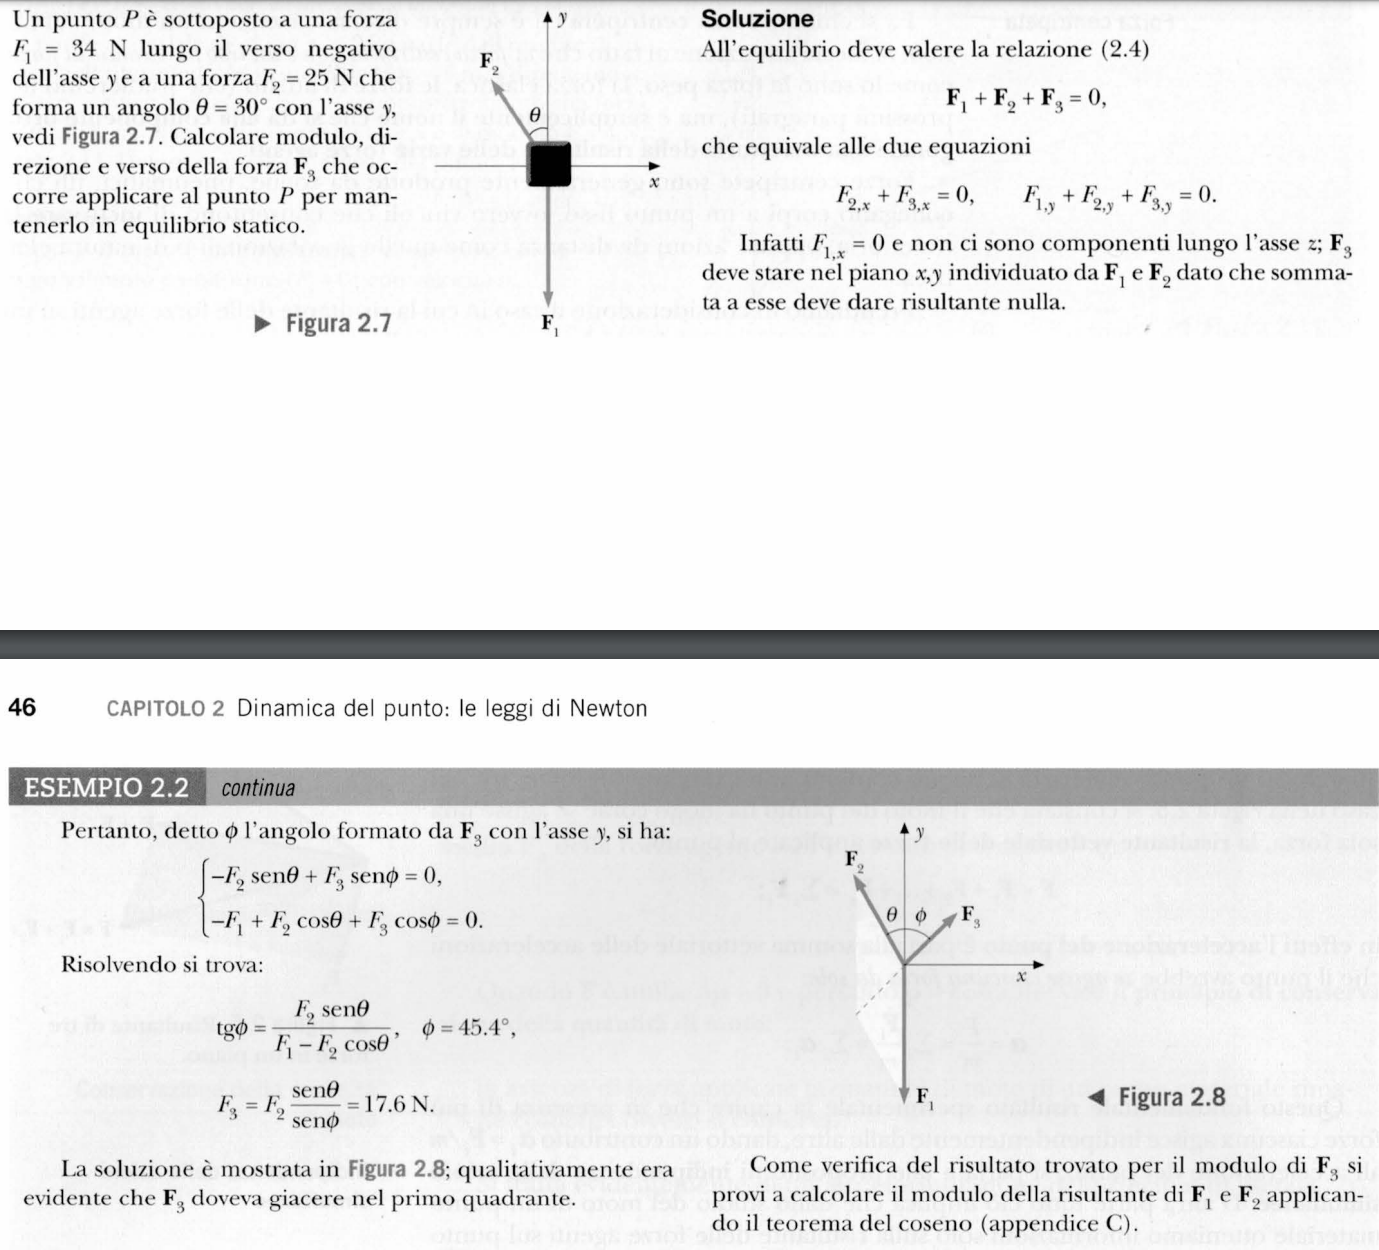
\includegraphics[width=0.7\textwidth]{2-2.png}
\end{figure}

\subsection{"Equilibrio dinamico"}
\begin{enumerate}
    \item moto rettilineo uniforme, $a = 0$, $\bar F = m\bar a = 0$
    \item moto rettilineo uniformemente accelerato, $a =$ costante
    \item moto curvilineo $\bar F = m\bar a_T + m\bar a_N = m\dfrac{dv}{dt} \bar u_T + m\dfrac{v^2}{R} \bar u_N$
\end{enumerate}
Si parla di equilibrio dinamico quando le forze che agiscono sul corpo provocano un moto uniforme e non accelerato.
\subsubsection{Esercizio 2.3}
\begin{figure}[H]
    \centering
    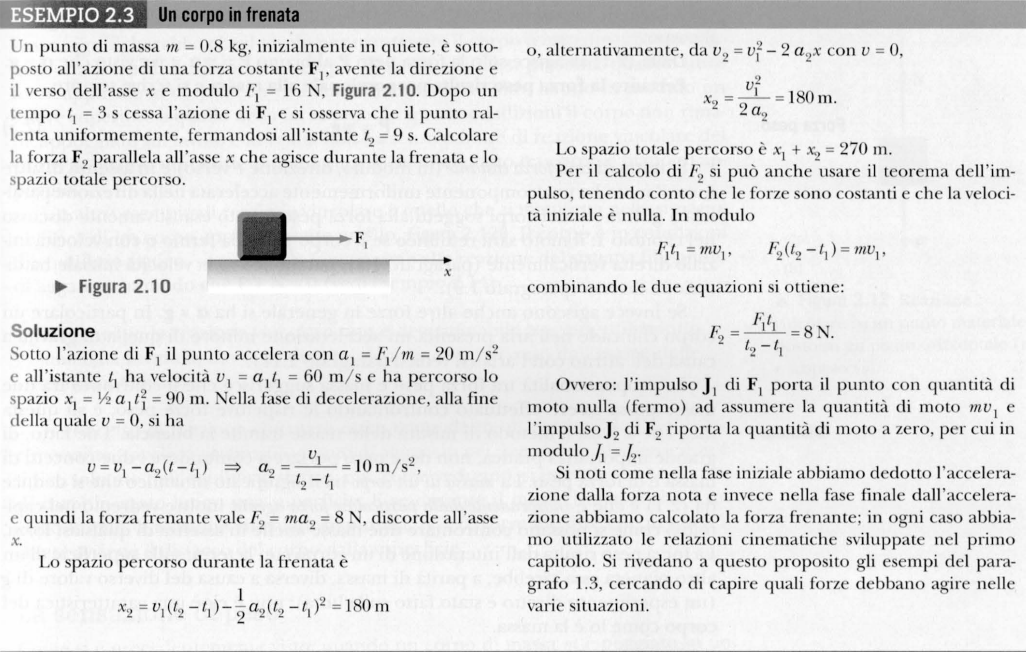
\includegraphics[width=0.7\textwidth]{2-3.png}
\end{figure}

\subsection{Forza Peso}
Il peso è la forza con cui la Terra attrae un corpo.
\[
    \vec P = m\vec g
\]
$1kg$ peso $\implies$ la forza con cui viene attratta la massa di $1kg$:
\[
    1Kg_p = 1Kg \cdot 9.81\dfrac{m}{s^2} = 9.81N
\]

\subsection{Reazione vincolare}
\begin{minipage}{0.6\textwidth}
    Se un corpo, soggetto all'azione di una forza o della risultante non nulla di un'insieme di forze rimane fermo, dobbiamo dedurre da quanto detto precendentemente che l'azione della forza provoca una reazione dell'ambiente circostante, detta \textbf{reazione vincolare}, che si esprime tramite una forza, eguale e contraria alla forza o alla risultante delle forze agenti, applicata al corpo stesso in modo tale che esso rimanga in quiete. Se prendiamo un oggetto che poggia su un tavolo, il tavolo esercita una forza uguale e contraria al peso del corpo, che si chiama reazione vincolare normale $\bar N$. Se si applicano ulteriori forze al corpo, la reazione vincolare deve equilibrare la risultante $\bar R$ di tutte le forze applicate al corpo.
    \[
        \bar R + \bar N = 0
    \]
\end{minipage}
\begin{minipage}{0.4\textwidth}
    \centering
    \begin{figure}[H]
        \centering
        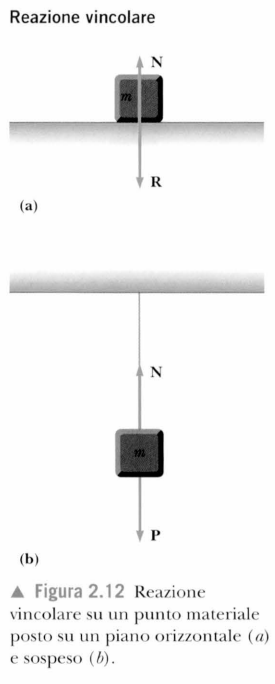
\includegraphics[width=0.3\textwidth]{reazione_vincolare.png}
    \end{figure}
\end{minipage}
\subsection{Sensazione di peso}
Come abbiamo appena visto, quando un corpo di massa $m$ è poggiato su un pavimento orizzontale, esso risente di una reazione vincolare $\bar N$ che in modulo vale $mg$. E' proprio questa reazione applicata al corpo che dà la \textit{sensazione di peso}. Prendiamo un corpo posato su una superficie che può muoversi verticalmente con un'accelerazione $\bar a$. Se il corpo rimane appoggiato sulla superficie la sue accelerazione è $\bar a$ e la sua equazione è:
\[
    \bar N + \bar P = m\bar a \ \ \implies \ \ \bar N + m\bar g = m\bar a \ \ \implies \ \ \bar N = m(\bar a - \bar g)
\]
perchè al corpo sono applicate sia la forza peso che la reazione dovuta al contatto con la superficie. Ora abbiamo quattro casi da esaminare; come asse di riferimento prendiamo un asse $z$ verticale orientato verso l'alto, per cui $\bar g = -g\bar u_z$:
\begin{enumerate}
    \item $\bar a$ discordante con $\bar g$, la superficie su cui è appogiato il corpo accelera verso l'alto
          \[
              \bar N = m[a\bar u_z - (-g\bar u_z)] = m(a + g)\bar u_z \ \ \implies \ \ N > mg
          \]
    \item $\bar a$ concorde con $\bar g$, la superficie su cui è appogiato il corpo accelera verso il basso, con $a < g$:
          \[
              \bar N = m[-a\bar u_z - (-g\bar u_z)] = m(a - g)\bar u_z \ \ \implies \ \ N > mg
          \]
    \item $\bar a = \bar g \ \ \implies \ \ \bar N = 0$: non c'è reazione e non c'è sensazione di peso
    \item $\bar a$ concorde con $\bar g$ con $a > g$: si ha il distacca del corpo dalla superficie.
\end{enumerate}
\subsubsection{Esercizio 2.5}
\begin{figure}[H]
    \centering
    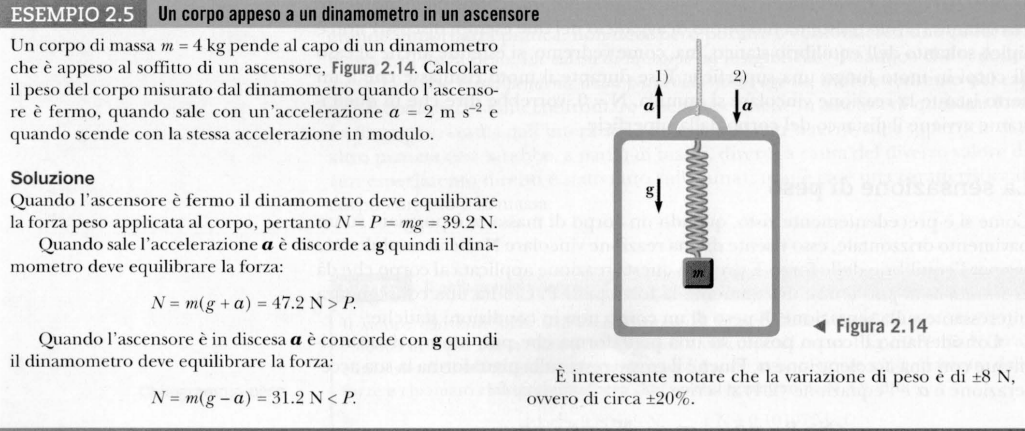
\includegraphics[width=0.7\textwidth]{2-5.png}
\end{figure}
\subsection{Forza di attrito}

\subsubsection{Forza di attrito radente}
\textbf{Forza di attrito statico} $F_s$: ci interessa il suo massimo in quanto è la forza che ostacola il moto. 
\[
    F_{s max} = \mu_s N \ \ \text{coefficiente di attrito statico}
\]
Quando il nostro corpo è già in movimento si parla di \textbf{attrito dinamico}:
\[
    F_d = \mu_d N
\]
dove $N = mg$. $F_d$ è costante fino a che si muove e $\mu_d < \mu_s$. La forza di attrito è sempre diretta in verso opposto alla velocità $\bar v$.\\
Una superficie si chiama \textbf{scabra} se c'è attrito o \textbf{liscia} se non c'è attrito.\\
Sul punto in movimento agisce una forza di attrito 
\[
   F_{ad} = -\mu N 
\]

\subsubsection{Esercizio 2.6}

\subsubsection{Esercizio 2.8}

\subsubsection{Esercizio 2.9}

\subsection{Piano inclinato}
Il piano inclinato è un piano che forma un angolo $\theta$ con l'orizzontale.
\begin{figure}[H]
    \centering
    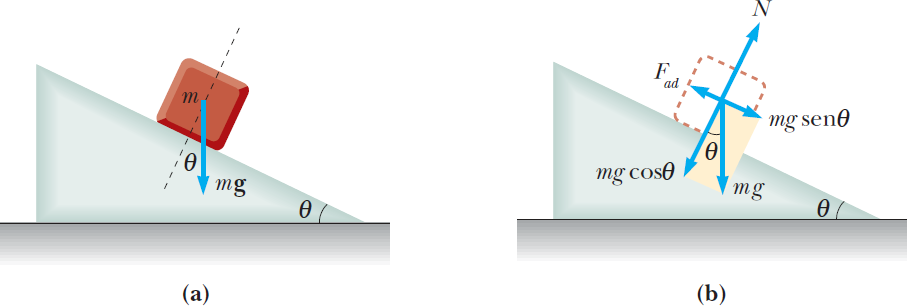
\includegraphics[width=0.5\textwidth]{piano_inclinato.png}
\end{figure}
\[
    N = mg\cos\theta \implies N - mg\cos\theta = 0
\]
Il corpo sta fermo fin quando la $\tan\theta < F_f$ (vedi da dove deriva)\\
La forza che fa scivolare il corpo è descritta da:
\[
    mg\sin\theta
\]
Mentre la forza di attrito:
\[
    F = \mu_d N \implies \mu_d \cdot mg\cos\theta
\]

\subsubsection{Esercizio 2.10}

\subsubsection{Esercizio 2.11}

\subsection{Forza di attrito viscoso}
La forza di attrito viscoso è una forza che si oppone al moto ed è proporzionale alla velocità del corpo soggetto a tale forza:
\[
    \bar F = -b\bar v
\]
dove $b$ è una costante che dipende dalla forma e dal mezzo.
\[
    m\dfrac{dv}{dt} = -b v \implies \int_{v_0}^{v}\dfrac{m}{v} dv = \int_{0}^{t} -b dt \implies \ln\dfrac{v}{v_0} = \dfrac{-b}{m}t \implies \dfrac{v}{v_0} = e^{-\dfrac{b}{m}t} \implies v = v_0 e^{-\dfrac{b}{m}t} \implies v = v_0 e^{-\dfrac{t}{\tau}} \ \ \ \text{dove} \ \ \ \tau = \dfrac{m}{b}
\]
Applicando la seconda legge di Newton
\[
    P + F = m\bar g - b\bar v = m\bar a = m\dfrac{d\bar v}{dt}
\]
La posizione iniziale del moto è nulla quindi il moto avviene solo lungo l'asse $z$, proiettiamo l'equazione su $z$:
\[
    \dfrac{dv}{dt} = g - \dfrac{bv}{m} \implies \dfrac{dv}{dt} = g - \dfrac{v}{\tau} \implies \dfrac{dv}{g - \dfrac{v}{\tau}} = dt \implies \int_{v_0}^{v} \dfrac{dv}{g - \dfrac{v}{\tau}} = \int_{0}^{t} dt \implies \ln\left(\dfrac{g- \dfrac{v}{\tau}}{g}\right) = -\dfrac{t}{\tau}
\]
Passando alle esponenziali otteniamo la velocità:
\[
    v(t) = g\tau\left(1-e^dfrac{-1}{\tau}\right)
\]
Inserisci le immagini per completezza
\subsection{Tensione dei fili}
Un filo può essere fissato in un estremo a un punto fisso e nell’altro a un punto materiale oppure può collegare due punti materiali. La forza che il filo esercita su qualisasi punto materiale è detta tensione del filo. Suporremo che la sua massa sia trascurabile e la lunghezza sia costante.

\subsection{Forza elastica, Oscillatore armonico semplice}
La molla è diversa dal filo. \\
Si definisce \textbf{forza elastica} una forza di direzione costante, con verso rivolto sempre a un centro $O$ e con modulo proporzionale alla distanza $r$ da $O$. Assumiamo come l'asse $x$ la direzione della forza e come origine il centro:
\[
    F = -kx \ \ \ \text{dove} \ \ \ k = \text{costante di molla}
\]
\[
    F = -ku_xx
\]
Limite di elasticità oltre il quale la molla si rompe/deforma.
\[
    m\bar a = -kx \implies m\dfrac{d^2x}{dt^2} = -kx \implies \dfrac{d^2x}{dt^2} = - \dfrac{k}{m}x \implies x = A\sin(\omega t + \phi) \ , \ \omega = \sqrt{\dfrac{k}{m}} \ \text{ moto armonico}
\]
\end{document}